% CLAUDE REPORT::WCD-SPACEFLOOR-0002::2026-11-14T15:30-08:00
% Claude routine "worst-case minimum derivation cost". User follow-up: overlay the space floors with the number of variables n.
% Role-neutral and additive. It does NOT edit root main.tex or any TMR/LSPV region.
\documentclass[11pt]{article}
\usepackage{amsmath,amssymb,amsthm,graphicx}
\usepackage[margin=1in]{geometry}
\newtheorem{theorem}{Theorem}
\title{WCD-SPACEFLOOR-0002: the space floors measured in the number of variables}
\author{Claude scheduled routine (worst-case derivation complexity log)}
\date{2026-11-14 15:30 America/Los\_Angeles}
\begin{document}
\maketitle

\paragraph{Status line.}
\begin{itemize}
\item Theorem~\ref{thm:dense} (sequential floor for density $m\approx n^{d}$): \textbf{PROVED/EXACT}, by the ONETAPE-0001 crossing-sequence argument with a denser padding block; family checks \textbf{COMPUTATIONAL}. Not independently reviewed.
\item Observation that no proved floor exceeds $S=n$: \textbf{PROVED/EXACT} for the floors in this report and WCD-SPACEFLOOR-0001.
\item P versus NP remains \textbf{OPEN}.
\end{itemize}

\section{Denser families}
Replace the padding block of the corpus equality family $F_{a,b}=A_a\,P_k\,B_b$ by $P^{(d)}$: $k^{d}$ distinct all-positive 3-clauses on $p$ fresh variables, $p$ minimal with $\binom p3\ge k^{d}$. Then $n=\Theta(k)$ (for $d\le3$), $L=\Theta(k^{d}\log k)$, the formula is satisfiable iff $a=b$, and all inputs of one size have one length.

\begin{theorem}\label{thm:dense}
A machine with a sequential two-way input head that decides 3-SAT in time $T$ and space $S$ satisfies, on this family,
\[T\cdot S\ \ge\ \Omega(k\cdot|P^{(d)}|)=\Omega(n^{d+1}\log n).\]
In variable units, with $T=n^{\tau}$ and $\tau\ge d$ (reading the input), $S\ge n^{\,d+1-\tau}$ up to logarithms. In input-length units, $S\ge L^{\,1+1/d-c}$ for $T=L^{c}$.
\end{theorem}
\begin{proof}
As in ONETAPE-0001 (source note 1): at each of the $|P^{(d)}|$ cuts inside the padding block, splicing shows that the $2^{k}$ satisfiable inputs $F_{a,a}$ need distinct crossing sequences, so for most $a$ the crossing sequence at that cut has length $\Omega(k/S)$. Summing over cuts bounds the time. Only the length of the padding block changed.
\end{proof}

\section{The overlay}
\begin{center}
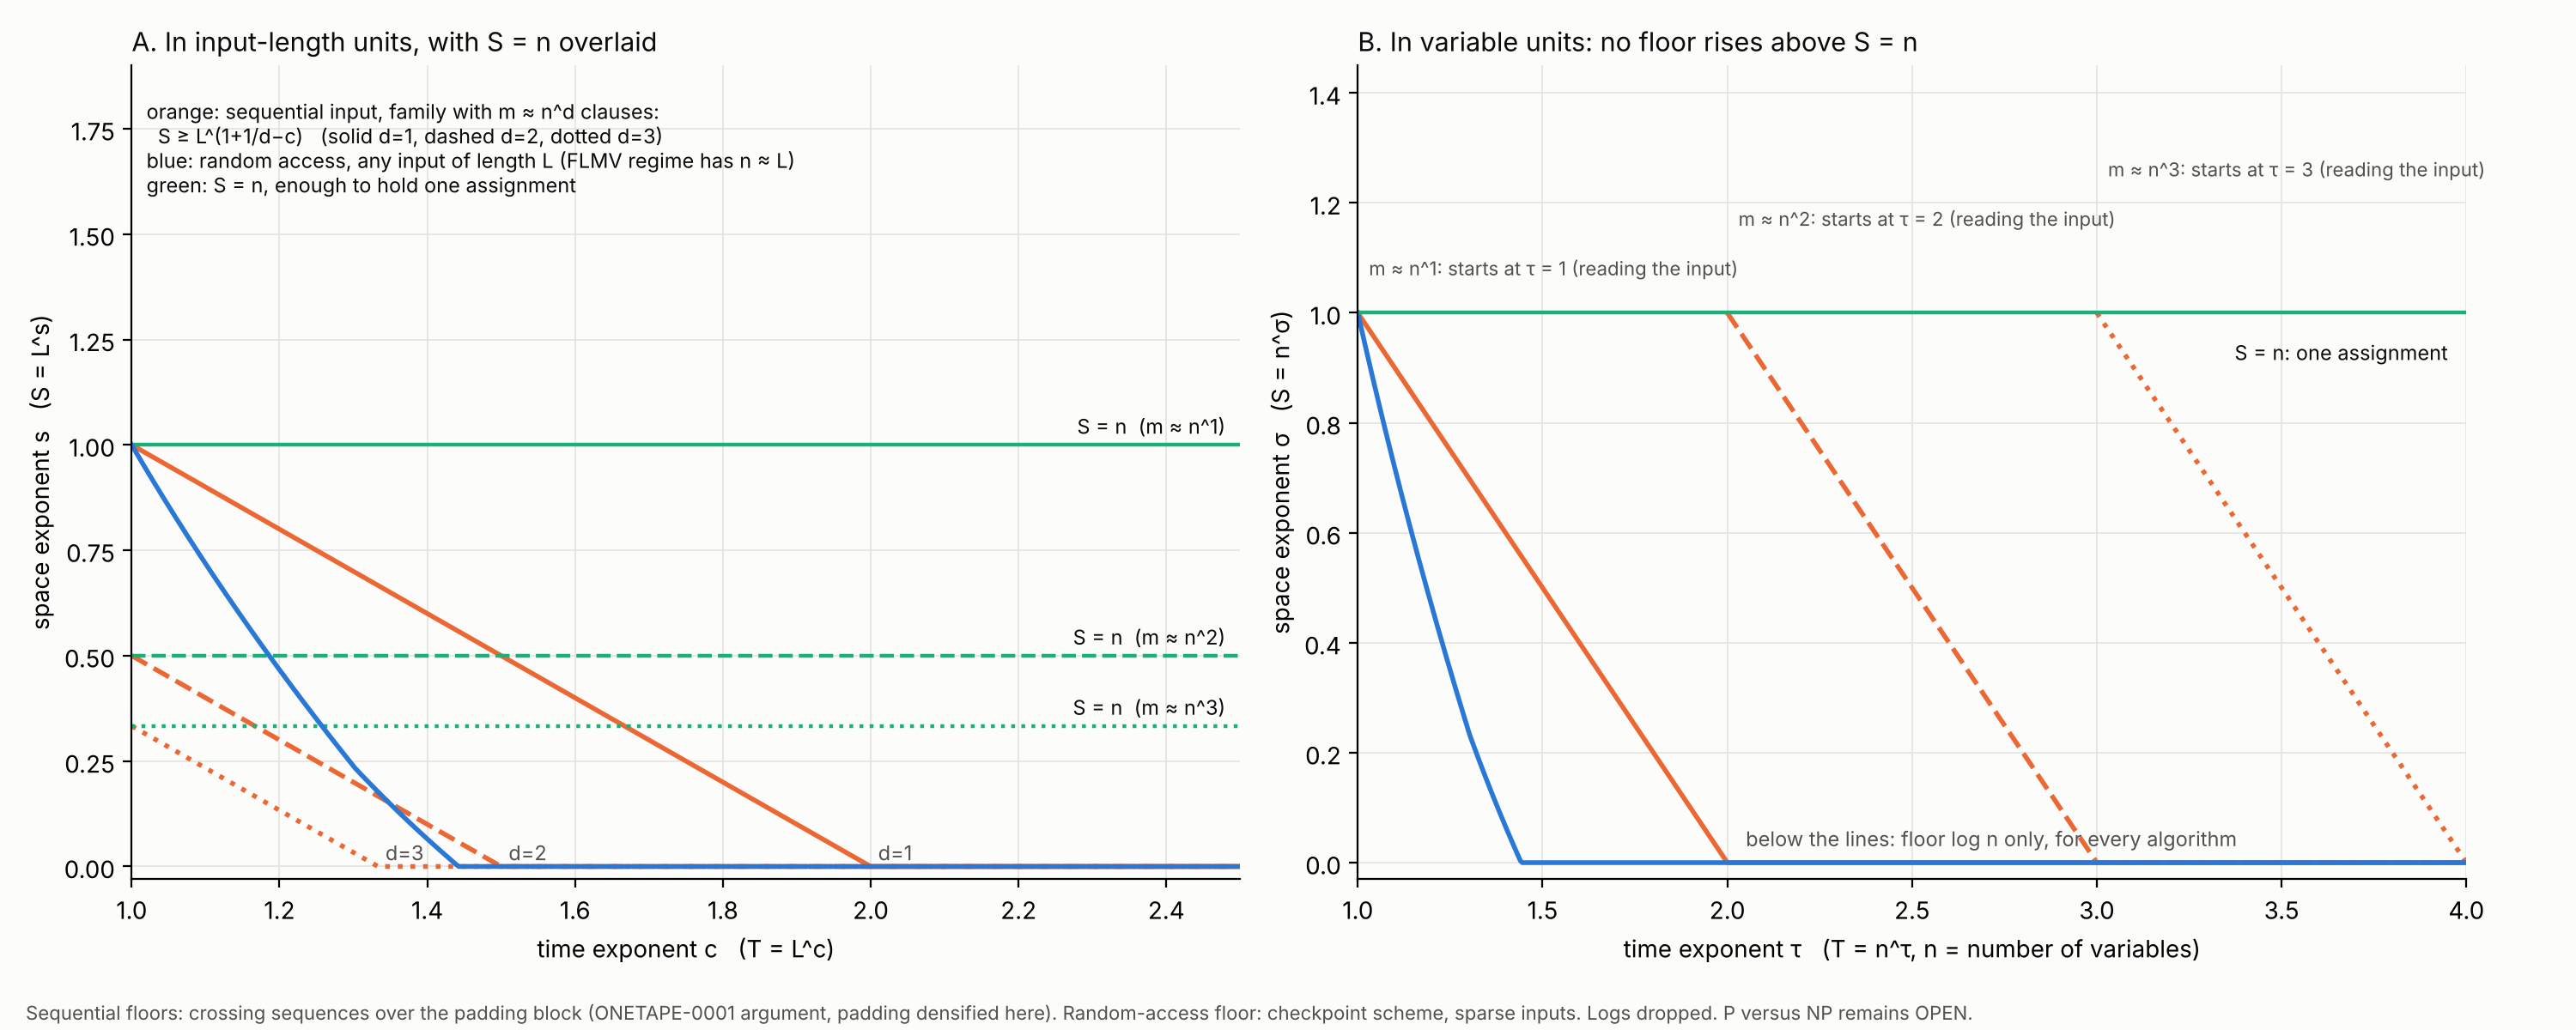
\includegraphics[width=\textwidth]{spacefloor/space_floor_n.png}
\end{center}
\begin{itemize}
\item \textbf{Panel A} (input-length units). The green lines mark $S=n$, the space needed to hold one full assignment, which sits at $s=1/d$ for density $m\approx n^{d}$. Each orange floor starts exactly on its green line at $c=1$ and falls below it.
\item \textbf{Panel B} (variable units). Each density starts at $\tau=d$, where merely reading the input costs $n^{d}$, with floor $S\approx n$, and falls to $\log n$ at $\tau=d+1$. Denser families keep the floor alive to larger time exponents, but no floor ever rises above $S=n$.
\end{itemize}

\paragraph{Reading.} Every proved space floor, at every running time, is at most the space needed to write down one assignment. In this sense the known bounds never force an algorithm to remember more than a single candidate solution, while brute force needs exactly that much space (with exponential time). A floor above $S=n$ for some polynomial time bound would say that fast algorithms must keep information about many assignments at once; no such statement is known, for any input model.

\section{CORPUS REVIEWED / DUPLICATION AUDIT / CHANGES}
\begin{itemize}
\item \textbf{Corpus reviewed:} WCD-SPACEFLOOR-0001; ONETAPE-0001 and its source notes; the consolidated living log.
\item \textbf{Duplication / contradiction audit:} the density variation is not in the corpus; the argument is ONETAPE-0001's. No contradiction found.
\item \textbf{What changed relative to root main:} nothing; \texttt{main.tex} is not edited.
\item \textbf{Adopted:} ONETAPE-0001. \textbf{Rejected / retired:} none.
\item \textbf{Stale or overstated claims found:} none.
\end{itemize}

\section{Evidence}
\texttt{spacefloor/space\_floor\_n.py}: exhaustive check for $k\le3$, $d=1,2,3$ (satisfiable iff $a=b$, one length per size); fitted growth $n\sim k^{0.97..0.99}$ and $L\sim n^{1.19,\,2.07,\,3.16}$ for $d=1,2,3$ at $k\le128$ (log factors included); figure \texttt{spacefloor/space\_floor\_n.png}. Output \texttt{spacefloor/raw\_results\_n.json}. No TeX engine was available, so this file was not compiled.

\medskip\noindent P versus NP remains OPEN. One OPEN load-bearing arrow means P $\ne$ NP is not proved.
\end{document}
% END_OF_VERIFIED_REPORT::CLAUDE::WCD-SPACEFLOOR-0002
